For CSS hovedenheden er udviklet en række diagrammer ud fra applikationsmodel metoden.
Der er et sekvensdiagram på figur \ref{fig:CSS_hovedenhed_SD} for alle de aktuelle use-cases som beskriver systemets virkemåde.
Ud fra dette er der lavet et klassediagram på figur \ref{fig:CSS_hovedenhed_Class} som dækker de forskellige use-cases med controller klasser og kommunikationenen til PC via RS232 og X10 Udtag via X10.


\begin{figure}[!htb]
	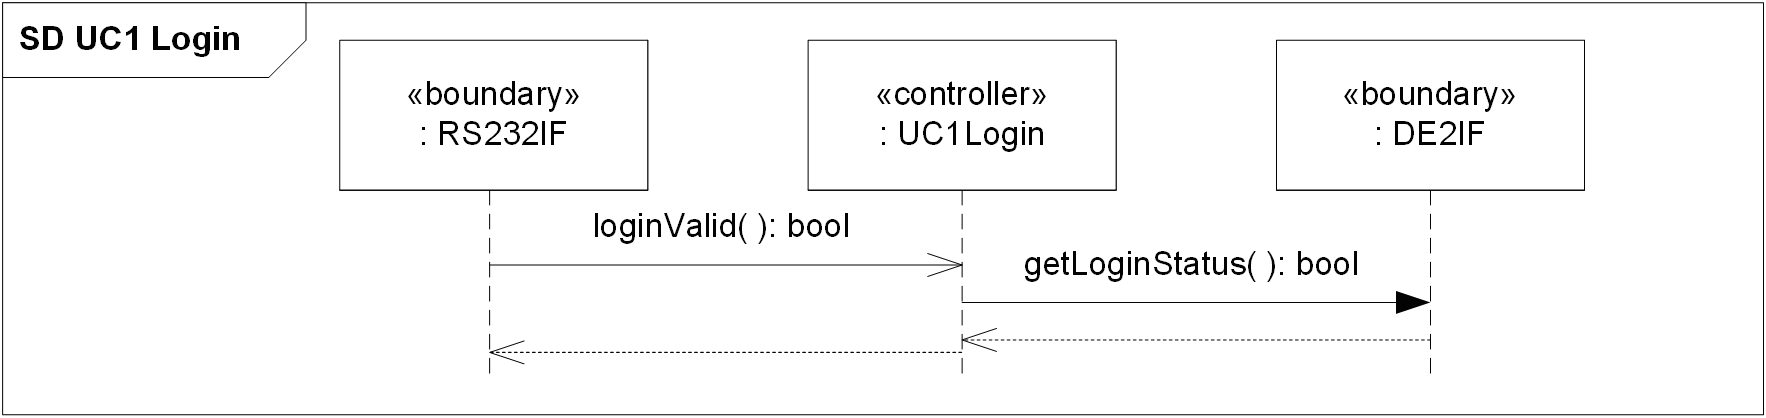
\includegraphics[width=\textwidth]{billeder/uml/CSS_hovedenhed_SD}
     \caption{Use-case sekvensdiagrammer for CSS hovedenhed}
     \label{fig:CSS_hovedenhed_SD}
\end{figure}

\begin{figure}[!htb] \centering
     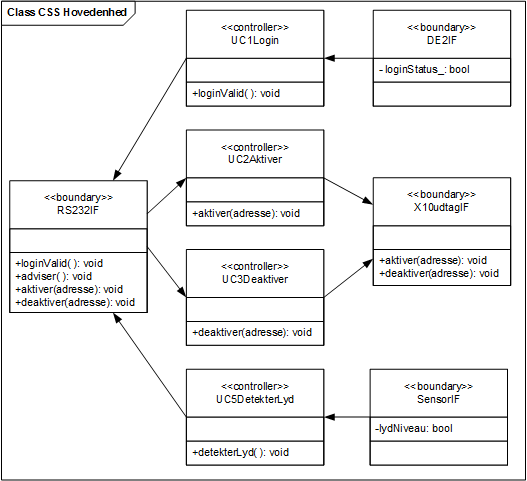
\includegraphics[width=0.8\textwidth]{billeder/uml/CSS_hovedenhed_Class}
     \caption{Klassediagram for CSS hovedenhed}
     \label{fig:CSS_hovedenhed_Class}
\end{figure}

Klasse diagrammet er dog kun et udkast, da den endelige implementering vel medføre en række støtte funktionaliteter. Da det er udvikling til en microcontroller er der også det hardware mæssige aspekt som resulterer i en række global funktioner som kan tilgåes fra hardwarenære funktioner. På figur \ref{fig:CSS_hovedenhed_Class_Static} ses det endelige diagram.